\documentclass{beamer}
\usepackage{handout}
\title{}
\author{}
\date{}
\begin{document}
\fontspec{Times New Roman}
\begin{frame}
\begin{center}
\Large{Chapter 1 Introduction to Politics} \\
\vspace{3em}
\normalsize{Instructor: Tzu-Chi Hsiao} \\
\vspace{3em}
\small{Department of Political Science} \\
\vspace{1em}
\small{National Taiwan University} \\
\end{center}
\end{frame}
\begin{frame}{Mutual Encouragement}
\begin{center}

\includegraphics[width=0.4\textwidth]{mc.png}
\end{center}
\begin{center}
學而不思則罔,思而不學則殆。 \\
Learning without thought puts effort in vain. Thought without learning leads to waste. 
\end{center}
\flushright Confucius
\end{frame}
\begin{frame}{Angel or Demon}
\begin{minipage}{0.4\textwidth}
\begin{center}

\includegraphics[width=\textwidth]{heal.png}
\end{center}
\begin{center}
May be an angel in the your grade.
\end{center}
\end{minipage}
\hfill
\begin{minipage}{0.4\textwidth}
\begin{center}
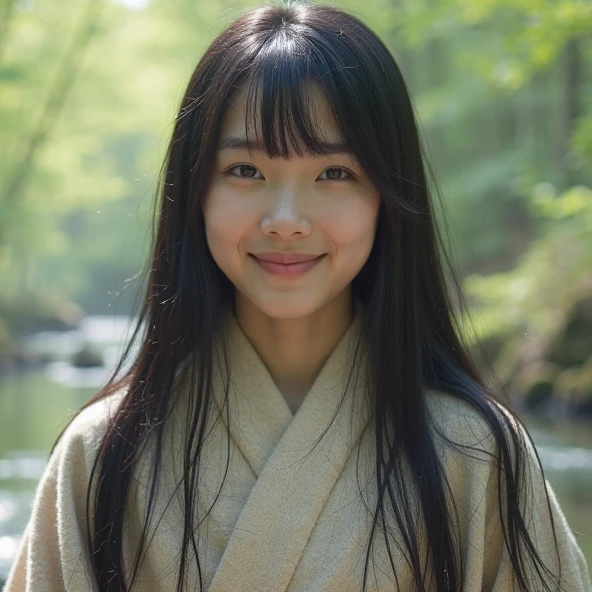
\includegraphics[width=\textwidth]{kill.png}
\end{center}
\begin{center}
May be a demon in the examination.
\end{center}
\end{minipage}
\end{frame}
\begin{frame}{Content}
\begin{itemize}
\item What is Politics?
\item The Political System
\item The State
\item The Nation
\item The Government
\end{itemize}
\end{frame}
\begin{frame}{Content}
\begin{itemize}
\item What is Politics?
\item \textcolor{gray}{The Political System}
\item \textcolor{gray}{The State}
\item \textcolor{gray}{The Nation}
\item \textcolor{gray}{The Government}
\end{itemize}
\end{frame}
\begin{frame}{Semi-Presidential System}
\begin{center}
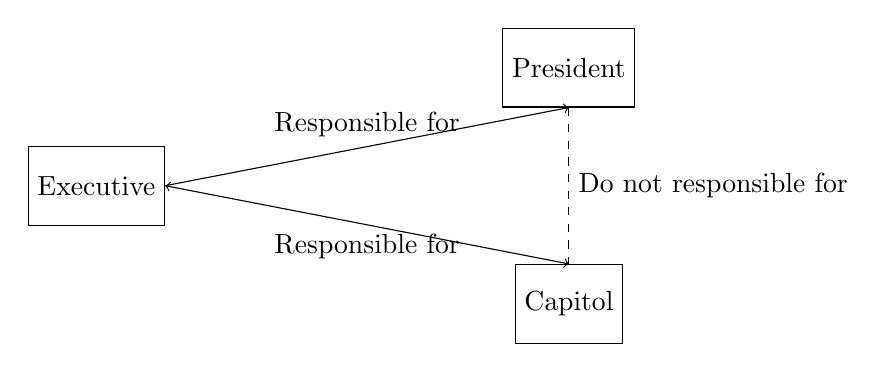
\begin{tikzpicture}
\node[draw, rectangle, minimum width=1cm, minimum height=1cm] (left) at (2, 0) {Executive};
\node[draw, rectangle, minimum width=1cm, minimum height=1cm] (topRight) at (8, 1.5) {President};
\node[draw, rectangle, minimum width=1cm, minimum height=1cm] (bottomRight) at (8, -1.5) {Capitol};
\draw[->] (left.east) -- (topRight.south) node[midway, above] {Responsible for};
\draw[<->] (left.east) -- (bottomRight.north) node[midway, below] {Responsible for};
\draw[dashed] (topRight.south) -- (bottomRight.north) node[midway, right] {Do not responsible for};
\end{tikzpicture}
\end{center}
\begin{center}
Figure I: An example of Semi-Presidential System.
\end{center}
\end{frame}
\begin{frame}{R.O.C. Semi-Presidential System}
\begin{center}
\begin{tikzpicture}
\node[draw, rectangle, minimum width=1cm, minimum height=1cm] (bottomLeft) at (6, -1.5) {Judicial Yuan};
\node[draw, rectangle, minimum width=1cm, minimum height=1cm] (topLeft) at (4, 1.5) {Supervisor Yuan};
\node[draw, rectangle, minimum width=1cm, minimum height=1cm] (left) at (2, 0) {Examinator Yuan};
\node[draw, rectangle, minimum width=1cm, minimum height=1cm] (topRight) at (10.5, 1.5) {Executive Yuan};
\node(1) at (4.5, -1.5) {}; \node(2) at (4.5, -2.5) {}; \node(3) at (6, -2.5) {}; % Empty nodes to implement the back-selfing line.
\node[draw, circle, minimum size=0.3cm] (circleleft) at (2, -1.5) {銓敘部};
\node[draw, rectangle, minimum width=1cm, minimum height=1cm] (bottomRight) at (9, -1.5) {Capitol};
\draw[<->] (topRight.west) -- (bottomRight.north) node[midway, right] {Responsible for};
\draw[->] (topLeft.east) -- (bottomRight.north) node[midway, left] {Supervisor to};
\draw[->] (topLeft.east) -- (topRight.west) node[midway, below] {Supervisor to};
\draw[-] (bottomLeft.west) -- (1.center) (1.center) -- (2.center) (2.center) -- (3.center); % Back-selfing line. Thanks to Prof. Chih-Jen, Lin.
\draw[->] (3.center) -- (bottomLeft.south) node[midway, right] {Check};
\end{tikzpicture}
\end{center}
\begin{center}
Figure II: An example of R.O.C. Semi-Presidential System. \\
\flushleft \tiny{Thanks to Prof. Rong-Hsiang, Tsay}
\end{center}
\end{frame}
\begin{frame}{Endeavor or Laid flat}
\begin{center}
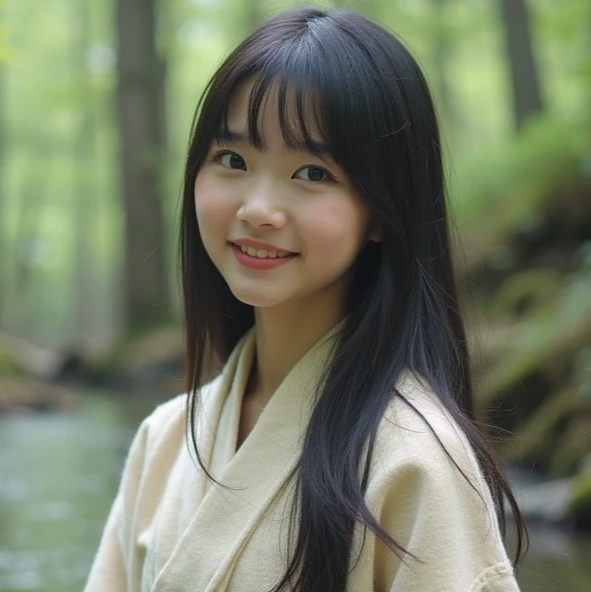
\includegraphics[width=0.4\textwidth]{fail.png}
\end{center}
\begin{center}
Endeavor is the key to success, unless you want to date with me.
\end{center}
\end{frame}
\begin{frame}{Good luck}
\begin{center}
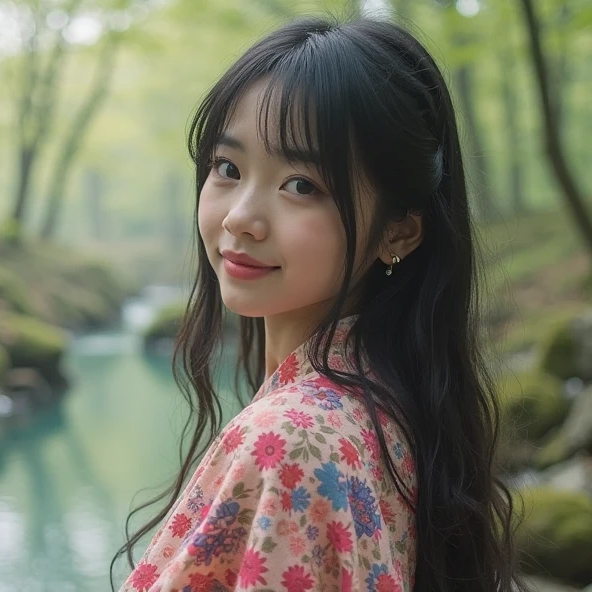
\includegraphics[width=0.4\textwidth]{good_luck.png}
\end{center}
\begin{center}
Good luck to all of you.
\end{center}
\end{frame}
\begin{frame}{}
\begin{center}
\Large{End of Chapter 1}
\end{center}
\end{frame}
\end{document}
